\def\baselinestretch{1}
\chapter{Database} \label{db}
\def\baselinestretch{1.66}

\noindent Come sopracitato, è stato utilizzato SQLite in quanto la natura embedded permette di incorporarlo direttamente nell'applicazione, rendendo la gestione dei dati più agevole e contribuendo a ridurre la complessità della configurazione del sistema. Questo è particolarmente vantaggioso per un'applicazione di medie dimensioni come la nostra.\\
\noindent Segue il diagramma relazionale del database impiegato come fondamento per la memorizzazione a lungo termine dei dati del software.

\begin{figure}[h]
\centering
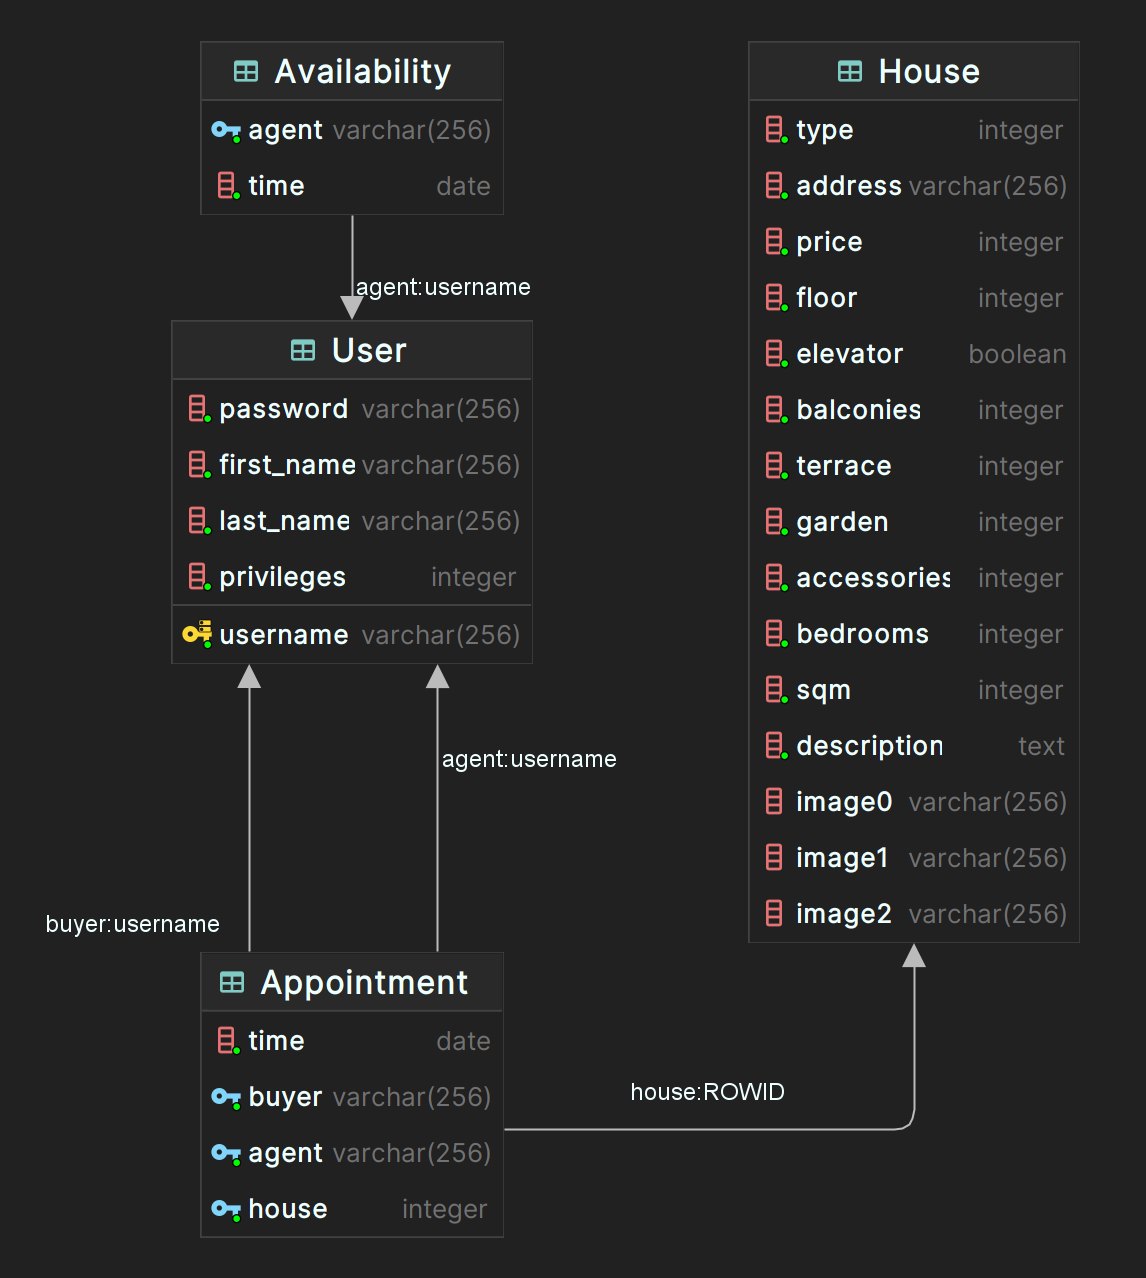
\includegraphics[scale=0.3]{properteaseDB.png}
\caption{Diagramma relazionale del database}
\end{figure}